\documentclass[10pt,twocolumn]{article}
\usepackage[utf8]{inputenc}
\usepackage{newtxtext}
\usepackage{newtxmath}
\usepackage{spverbatim}
\usepackage{graphicx}
\usepackage{icomma}
\usepackage{listings}
\usepackage{xcolor}
\usepackage{color}
\hyphenation{au-to-kor-re-la-ti-on}
\definecolor{dkgreen}{rgb}{0,0.6,0}
\definecolor{gray}{rgb}{0.5,0.5,0.5}
\definecolor{mauve}{rgb}{0.58,0,0.82}

\lstset{%
    aboveskip=3mm, belowskip=3mm,
    showstringspaces=false,
    columns=flexible,
    basicstyle={\small\ttfamily},
    numbers=none,
    numberstyle=\tiny\color{red},
    keywordstyle=\color{blue},
    commentstyle=\color{dkgreen},
    stringstyle=\color{mauve},
    breaklines=true,
    breakatwhitespace=true,
    tabsize=3
}

\renewcommand{\figurename}{Figur}

\raggedbottom{}
\sloppy

\title{Laborationsrapport i TSKS10 \emph{Signaler, Information och Kommunikation}}

\author{Malcolm Vigren \\ malvi108, 19950127--0970 }

\date{16 maj, 2017}

\begin{document}

\maketitle

\section{Inledning}

Syftet med denna laboration var att I/Q-demodulera och behandla en radiosignal
för att kunna höra vad som sändes. Enligt problemformuleringen skickar
radiostationen signalen:
\begin{align*}
    x(t) = x_I(t)\cos(2 \pi f_c t) - x_Q(t)\sin(2 \pi f_c t) + w(t) + z(t)
\end{align*}
där $x_Q(t)$ och $x_I(t)$ är de meddelanden som skulle lyssnas efter. 
Båda innehöll två olika melodier samt varsitt ordspråk som skulle identifieras.
$f_c$ är signalens bärfrekvens, $z(t)$ är en summa av andra I/Q-modulerade
signaler och $w(t) = 0,001(\cos(2 \pi f_1 t) + \cos(2 \pi f_2 t))$, där $f_1$ och
$f_2$ ligger långt ifrån bärfrekvenserna hos de andra signalerna. En del av
uppgiften var att ta reda på $f_c$, $f_1$ och $f_2$. $f_c$ var enligt
problemformuleringen en av följande frekvenser: 18, 37, 56, 75, 94, 113,
132, 151 kHz.

På grund av utformningen av miljön innehåller den mottagna signalen en
ekoeffekt, sådan att vi tar emot signalen:
\begin{align*}
    y(t) = x(t - \tau_1) + 0,9x(t - \tau_2)
\end{align*}
En del av uppgiften var att ta reda på skillnaden i fördröjning mellan 
de olika signalerna,
alltså $\tau_2 - \tau_1$. Denna var enligt problemformuleringen mindre än 500 ms
och en multipel av 1 ms.

Signalen tillhandahölls i form av en \textit{wav}-fil med sampelfrekvensen 400kHz.

\section{Metod}

Uppgiften löstes med programmeringsspråket \textit{Python}, tillsammans med
biblioteken \textit{numpy}, \textit{scipy} och \textit{matplotlib}.

\subsection{Letande av kandidater till $f_c$ och bestämmande av $f_1$ och
$f_2$}\label{sub:candidates}

För att ta reda på $f_c$ fouriertransformerades signalen i wav-filen, och
amplitudspektrumet plottades, se Figur~\ref{fig:yamp}. 
\begin{figure}[h]
    \centering
    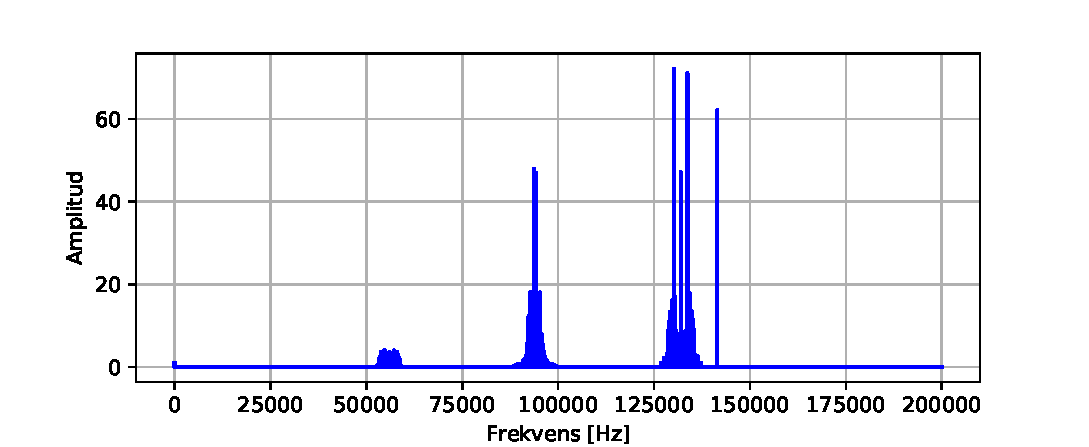
\includegraphics[width=\linewidth]{figures/yamp.pdf}
    \caption{Amplitudspektrum för $y(t)$}\label{fig:yamp}
\end{figure}
Från detta kunde en del kandidater till $f_c$ uteslutas, sådan att
de möjliga värdena var 56, 94, 132 kHz, då det är runt dessa frekvenser de
olika signalerna samlades runt. Från detta kunde också frekvenserna för
cosinussignalerna från $w(t)$
bestämmas, då dessa var två mycket närliggande spikar vid 141500 respektive
141501 Hz. Alltså är $f_1=141500$ Hz och $f_2=141501$ Hz.

\subsection{Bestämmande av $\tau_2 - \tau_1$}
För att bestämma fördröjningen $\tau_2 - \tau_1$ användes autokorrelation. För
att göra detta utnyttjades det faktum att $\tau_2$ sekunder in i signalen
hörs inget eko, vilket betyder att man kan använda signalen fram till $\tau_d$
sekunder som det som ska korreleras, för något $\tau_d < \tau_2 - \tau_1$.

Vi betecknar signalvärdet vid sampel $n$ som $y_n$. Vidare definierar vi korrelationen
$z(\tau)$ som, där $f_s$ är sampelfrekvensen:

\begin{equation*}
    z(\tau) = \frac{1}{f_s}\sum_{i=0}^{\tau_d f_s}y_iy_{i + \tau f_s}
\end{equation*}

Detta gör att $z(\tau)$ blir ett mått på hur början av $y(t)$ ($y(t)$ för $0
\leq t \leq \tau_d$)
"passar" med hela $y(t)$ när det är förskjutet med $\tau$ sekunder. Vi
borde därför se en topp i $z(\tau)$ vid $\tau = 0$, eftersom signalerna är identiska då, och en mindre topp där $\tau
= \tau_2 - \tau_1$, eftersom det är då ekot börjar.

$\tau_d$ valdes till 0.25 sekunder. Signalen som skulle korreleras valdes till
signalen med bärfrekvensen 56 kHz i Figur~\ref{fig:yamp}, eftersom denna hade
en vågform som liknade vitt brus. Denna filtreras ut med ett bandpassfilter och
$z(\tau)$ beräknades för $0 \leq \tau < 500$ ms, se Figur~\ref{fig:corr}.

\begin{figure}[h]
    \centering
    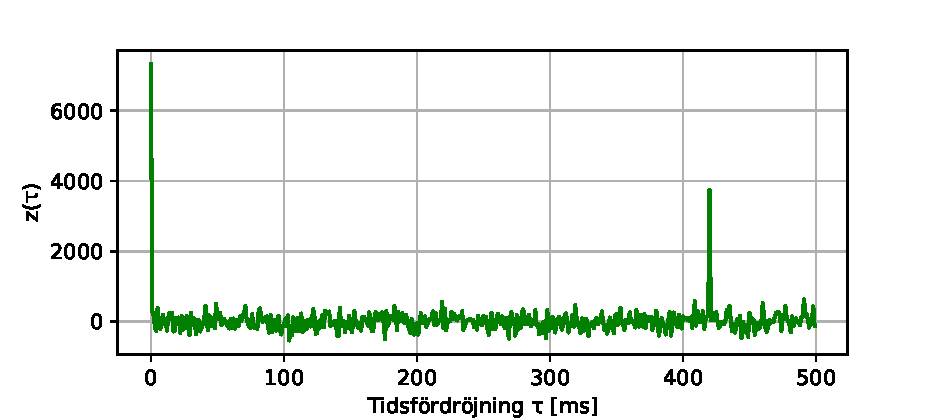
\includegraphics[width=\linewidth]{figures/corr.pdf}
    \caption{Korrelationen $z(\tau)$}\label{fig:corr}
\end{figure}

Avläsning ur grafen för $z(\tau)$ visade en topp vid $\tau = 420$ ms, vilket
betydde att $\tau_2 - \tau_1 = 420$ ms.

\subsection{Borttagning av eko}\label{sub:echo}
Värdet på $\tau_2 - \tau_1$ utnyttjades för att ta bort ekoeffekten från signalen. Vi
vet från problemformuleringen att ekot var 0,9 gånger så starkt som resten av signalen 
och att den dröjde med $\tau_2 - \tau_1$ sekunder. För att ta bort ekoeffekten
användes $y_0(t) = y(t) - 0,9y_0(t - (\tau_2 - \tau_1))$ för alla $t > \tau_2
- \tau_1$, där $y_0(t)$ är signalen
utan ekoeffekt. Detta implementerades med en \textit{for-loop}.
% För
% att ta bort ekot subtraherades helt enkelt ekot bort genom att för varje
% sampel subtrahera med det värde $\tau_2 - \tau_1$ sekunder bak i tiden multiplicerat
% med 0.9, vilket gjordes med hjälp av en \textit{for-loop}.

% Denna procedur kördes
% nu innan I/Q-demoduleringen, vilket gjorde innehållet av radiosignalen
% tillräckligt hörbar för att identifiera ordspråken.

% \subsection{Bestämmande av $\delta$\label{sub:delta}}
% 
% Fel värde på $\delta$ gör att $x_I(t)$ och $x_Q(t)$ blandas efter
% demodulationen. Optimalt värde på $\delta$ är alltså det värde som gör att man
% inte alls kan höra I-komponenten i Q-komponenten och vice versa. För att ta
% reda på detta $\delta$ kördes I/Q-demodulerings- och ekoborttagningsrutinen på
% flera olika värden på $\delta$, $0 \leq \delta < \frac{\pi}{2}$ i steg om
% $0.05\pi$, och manuellt lyssnade på resultaten. Det visades att $0.25\pi$ gav
% ett nästan perfekt resultat, vidare prövning gav att $\delta = 0.24\pi$ gav den
% bästa separationen av $x_I(t)$ och $x_Q(t)$. Nu var signalerna så klara att
% ordspråken kunde identifieras.

\subsection{I/Q-demodulering\label{sub:iq}}
Innan demoduleringen bandpassfiltrerades $y_0(t)$, signalen med borttagen
ekoeffekt från Avsnitt~\ref{sub:echo}, runt en av kandidaterna
för bärfrekvenserna beskrivna i Avsnitt~\ref{sub:candidates} för att få bort de
ointressanta signalerna. Vi betecknar den filtrerade $y_0(t)$ som $\hat{y}(t)$.
För I/Q-demodulering av signalen användes sambanden

\begin{equation*}
    \hat{x}_I(t) = \mathcal{H}_{B/2}^{LP}\{2\hat{y}(t)\cos(2\pi f_c t + \delta)\}
\end{equation*}
\begin{equation*}
    \hat{x}_Q(t) = \mathcal{H}_{B/2}^{LP}\{-2\hat{y}(t)\sin(2\pi f_c t + \delta)\}
\end{equation*}

där $B$ är nyttosignalens bandbredd, avläst i Figur~\ref{fig:yamp} som 12 000
kHz, och
$\hat{x}_I(t)$ och $\hat{x}_Q(t)$ är de mottagna I- och Q-komponenterna som
idealt ska vara lika med $x_I(t)$ och $x_Q(t)$.
Konstanten $\delta$ representerar en kompensation för fasvridningen med 
$-2\pi f_c \tau_1$ radianer signalen har fått efter
att den skickats över kanalen, eftersom det har tagit $\tau_1$ sekunder för
signalen att nå mottagaren. Ett felaktigt värde på $\delta$ gör att
I- och Q-komponenterna blandas med varandra efter demoduleringen.

Först sattes $\delta = 0$ och signalen demodulerades för de olika
frekvensbanden för att ta reda på vilket som innehöll det intressanta ljudet. Det
visade sig att signalen med $f_c = 94$ kHz innehöll något som liknade det som
beskrevs av problemformuleringen, det sökta $f_c$ var alltså 94 kHz.
Nu kunde $\delta$ bestämmas, som prövades fram genom att demodulera signalen med olika $\delta$, och
lyssna på vilket $\delta$ gjorde att man inte kunde höra en del av I-komponenten i
Q-komponenten och vice versa. Endast värden mellan 0 och $\frac{\pi}{2}$ behövde prövas,
då större fasvridning leder till att signalerna i de demodulerade I- och Q-komponenterna byter plats.
Prövningen gav värdet $0.24\pi$. Demodulation med detta värde på $\delta$ gjorde
att ordspråken i meddelandena nu kunde identifieras i $\hat{x}_I(t)$ och
$\hat{x}_Q(t)$.

% För att demodulera signalen bandpassfiltrerades den för att extrahera
% signalen för en viss bärfrekvens. Detta gjordes genom att bestämma vilka
% frekvensband varje signal befann sig i från Figur~\ref{fig:yamp}, och använda
% ett digitalt butterworthfilter för att filtrera ut signalen. Den filtrerade
% signalel multiplicerades med $\mathcal{H}_{B/2}^{LP}\{2\cos(2\pi f_c t +
% \delta)\}$ och 
% $-2\sin(2\pi f_c t + \delta)$ 
% för att få ut $x_I(t)$- respektive $x_Q(t)$-komponenterna av signalen.

\section{Resultat}

Den sökta informationen är:
\begin{itemize}
\item Bärfrekvensen för nyttosignalen är $f_c=94$ kHz.
\item $f_1=141500$ Hz och $f_2=141501$ Hz
\item $\tau_2 - \tau_1 = 420$ ms.
\item Ordspråket i $x_I(t)$ är "Väck inte den björn som sover".
\item Ordspråket i $x_Q(t)$ är "Äpplet faller inte långt från trädet".
\end{itemize}

\clearpage

\onecolumn
\section*{Min Python-kod:}
\lstinputlisting[language=Python]{../python/main.py}

\end{document}
